\documentclass[11pt,letterpaper]{article}

\usepackage[margin=1in]{geometry}
\usepackage{graphicx}
\usepackage{subcaption}
\usepackage{booktabs}
\usepackage{hyperref}
\usepackage{parskip}
\usepackage{float}
\usepackage{microtype}
\usepackage{soul}
\usepackage{amsmath}

\hypersetup{colorlinks=true, linkcolor=blue, urlcolor=blue}

\title{\textbf{CS5330 Computer Vision: Project 5}\\
       \large Recognition using Deep Networks}
\author{Shriman Raghav Srinivasan}
\date{July 2026}

\begin{document}

\maketitle

% ============================================================
\section*{Project Overview}
% ============================================================

In this project, I explored deep learning architectures for image classification tasks. I built and trained a Convolutional Neural Network (CNN) from scratch to classify handwritten digits using the MNIST dataset. I then examined the learned representation by visualizing the weights of the first convolutional layer and applying these filters to input images. Following this, I applied transfer learning by freezing the CNN backbone and fine-tuning a new classification head on Greek letters, reaching perfect accuracy. I also implemented and trained a Vision Transformer (ViT) network on MNIST to compare self-attention mechanisms against local convolutions. Finally, I automated a hyperparameter sweep of 50 configurations to analyze how learning rate, optimizer selection, batch size, and activation functions influence CNN convergence speed and classification performance.

I completed this project entirely alone.

% ============================================================
\section*{Source Code}
% ============================================================

The full source code for this project is available at:\\
\url{https://github.com/shrirag10/CS5330-Pattern-Recognition-Computer-vision-/tree/main/Projects/project5}

Instructions for building and running the python scripts are in the \texttt{README.md} file in the project folder.

% ============================================================
\section*{Methodology and Results}
% ============================================================

%------------------------------------------------------------
\subsection*{Task 1: Digit Recognition CNN}
%------------------------------------------------------------

I designed and trained a custom Convolutional Neural Network model named \texttt{MyNetwork}. The network consists of:
\begin{itemize}
    \item \textbf{Conv1}: 1D grayscale input to 10 feature channels using 5x5 filters.
    \item \textbf{MaxPool1 + ReLU}: 2x2 max pooling followed by Rectified Linear Unit activation.
    \item \textbf{Conv2 + Dropout}: 10 channels to 20 channels using 5x5 filters, combined with a 0.5 dropout rate to prevent overfitting.
    \item \textbf{MaxPool2 + ReLU}: 2x2 max pooling followed by ReLU.
    \item \textbf{FC1 + ReLU}: Flattened features (320 nodes) projected to 50 hidden nodes, followed by ReLU.
    \item \textbf{FC2 + LogSoftmax}: 50 nodes projected to 10 output classes, normalized using LogSoftmax.
\end{itemize}

\begin{figure}[H]
    \centering
    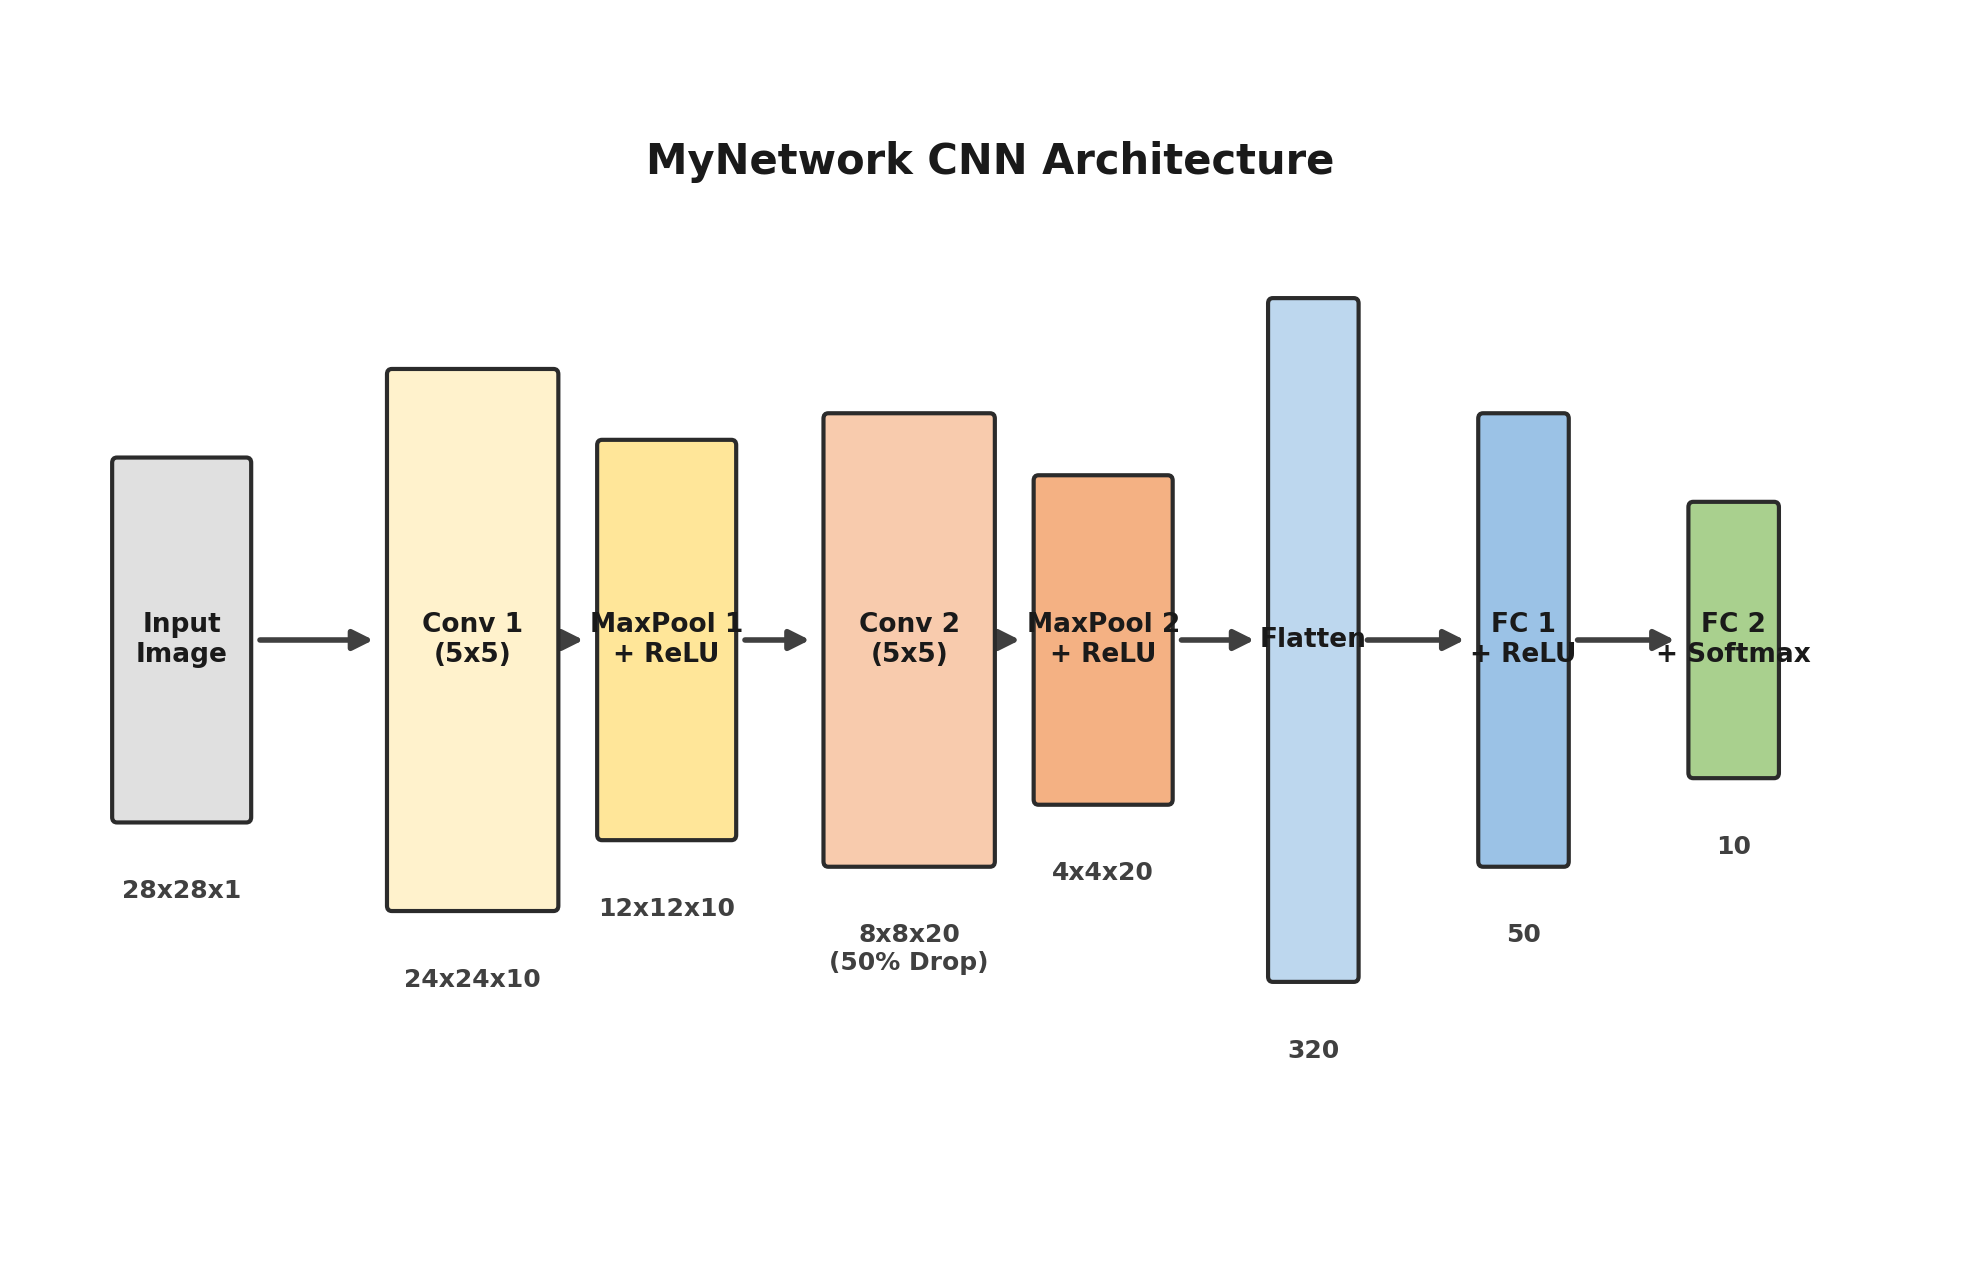
\includegraphics[width=0.85\textwidth]{network_diagram.png}
    \caption{Detailed architectural layout of MyNetwork CNN model showing layer dimensions.}
    \label{fig:network_diagram}
\end{figure}

I trained the network on the MNIST training dataset using Stochastic Gradient Descent (SGD) with a learning rate of $0.01$, momentum of $0.5$, and batch size of 64. The model was trained for 5 epochs on the GPU.

The first six example digits from the test set are displayed in Figure~\ref{fig:first_six_digits}.

\begin{figure}[H]
    \centering
    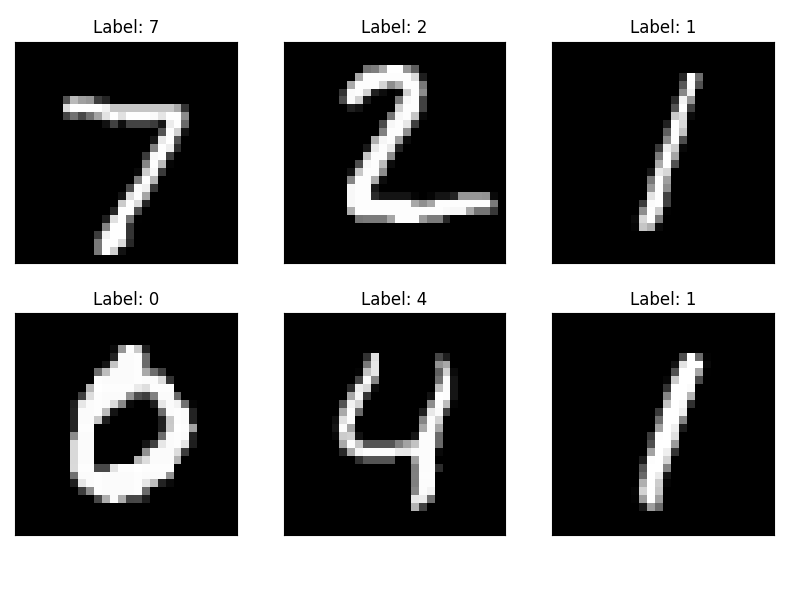
\includegraphics[width=0.6\textwidth]{first_6_test_digits.png}
    \caption{The first six example digit images from the MNIST test set.}
    \label{fig:first_six_digits}
\end{figure}

The training and testing loss/accuracy curves are shown in Figure~\ref{fig:task1_curves}. The model quickly converged, achieving a final test accuracy of \textbf{98.18\%} and a test loss of $0.0543$ at the end of epoch 5.

\begin{figure}[H]
    \centering
    \begin{subfigure}[b]{0.48\textwidth}
        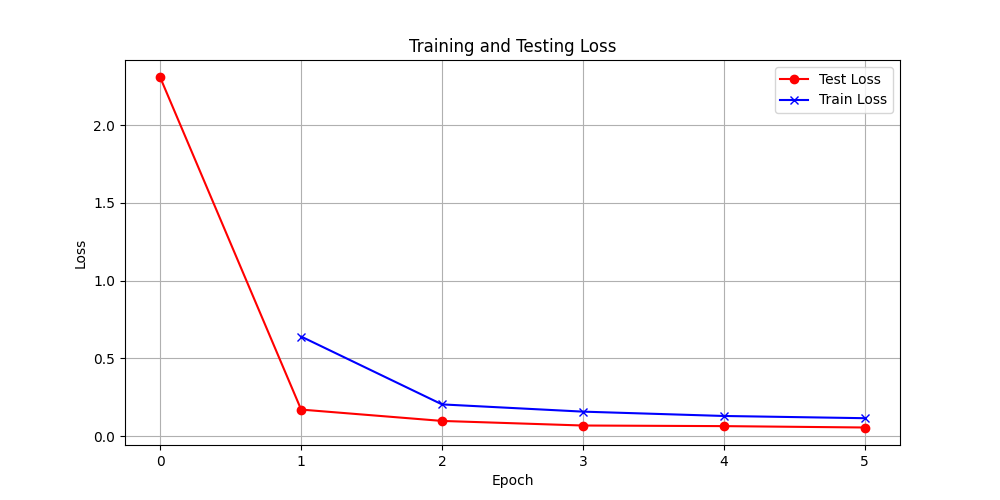
\includegraphics[width=\textwidth]{loss_plot.png}
        \caption{Loss Curves}
    \end{subfigure}
    \hfill
    \begin{subfigure}[b]{0.48\textwidth}
        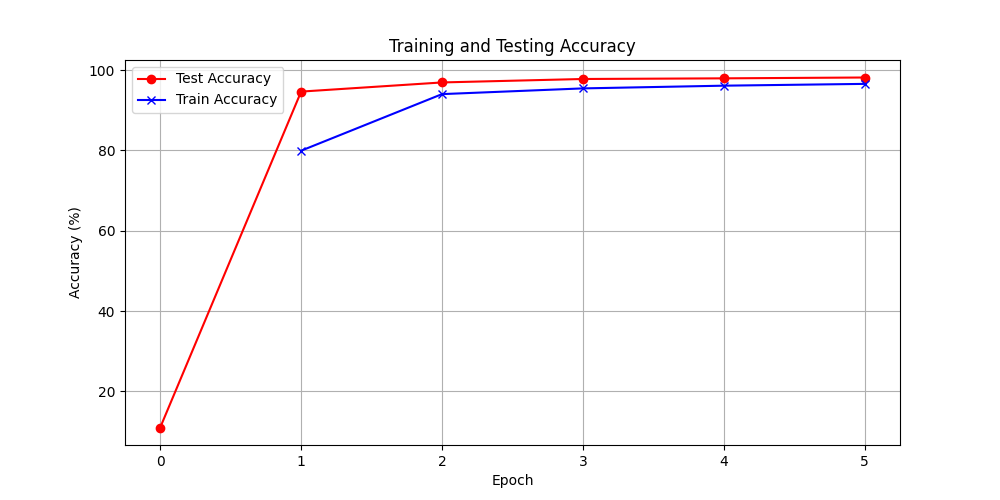
\includegraphics[width=\textwidth]{accuracy_plot.png}
        \caption{Accuracy Curves}
    \end{subfigure}
    \caption{MNIST CNN training and testing curves over 5 epochs.}
    \label{fig:task1_curves}
\end{figure}

To verify the model, I ran inference on the first 10 images of the test set. The model correctly predicted all 10 digits. The printed output values, predicted indices, and correct target labels are detailed in Table~\ref{tab:first_10_outputs}.

\begin{table}[H]
    \centering
    \caption{Log-probability outputs, predictions, and correct labels for the first 10 MNIST test images.}
    \label{tab:first_10_outputs}
    \small
    \begin{tabular}{@{}cccp{11.5cm}@{}}
        \toprule
        \textbf{Ex.} & \textbf{Target} & \textbf{Pred} & \textbf{Network Output Log-Probabilities [0 to 9]} \\ \midrule
        1 & 7 & 7 & [-17.70, -19.66, -10.53, -10.99, -25.85, -18.90, -33.66, \textbf{0.00}, -14.46, -13.95] \\
        2 & 2 & 2 & [-10.20, -9.08, \textbf{0.00}, -15.48, -21.69, -23.53, -14.30, -16.51, -12.14, -29.58] \\
        3 & 1 & 1 & [-13.16, \textbf{0.00}, -9.51, -12.18, -7.47, -14.60, -13.95, -7.34, -10.51, -11.19] \\
        4 & 0 & 0 & [\textbf{0.00}, -25.05, -11.98, -20.76, -20.34, -17.28, -12.02, -13.93, -16.21, -12.68] \\
        5 & 4 & 4 & [-15.96, -21.63, -13.85, -16.94, \textbf{0.00}, -16.00, -14.72, -13.51, -15.79, -6.56] \\
        6 & 1 & 1 & [-16.35, \textbf{0.00}, -11.77, -14.05, -8.24, -19.43, -18.96, -8.31, -11.73, -12.52] \\
        7 & 4 & 4 & [-28.79, -14.48, -16.57, -16.03, \textbf{0.00}, -14.13, -26.41, -12.67, -8.04, -8.43] \\
        8 & 9 & 9 & [-18.13, -15.22, -10.29, -9.02, -6.68, -9.81, -18.81, -9.35, -10.15, \textbf{0.00}] \\
        9 & 5 & 5 & [-12.39, -21.98, -13.92, -16.92, -12.62, \textbf{-0.01}, -4.83, -15.95, -6.58, -6.98] \\
        10 & 9 & 9 & [-21.50, -23.14, -16.68, -12.81, -9.05, -17.87, -28.08, -5.60, -8.72, \textbf{0.00}] \\ \bottomrule
    \end{tabular}
\end{table}

The program also plotted the first 9 digits in a grid along with their predicted labels (Figure~\ref{fig:task1_preds}).

\begin{figure}[H]
    \centering
    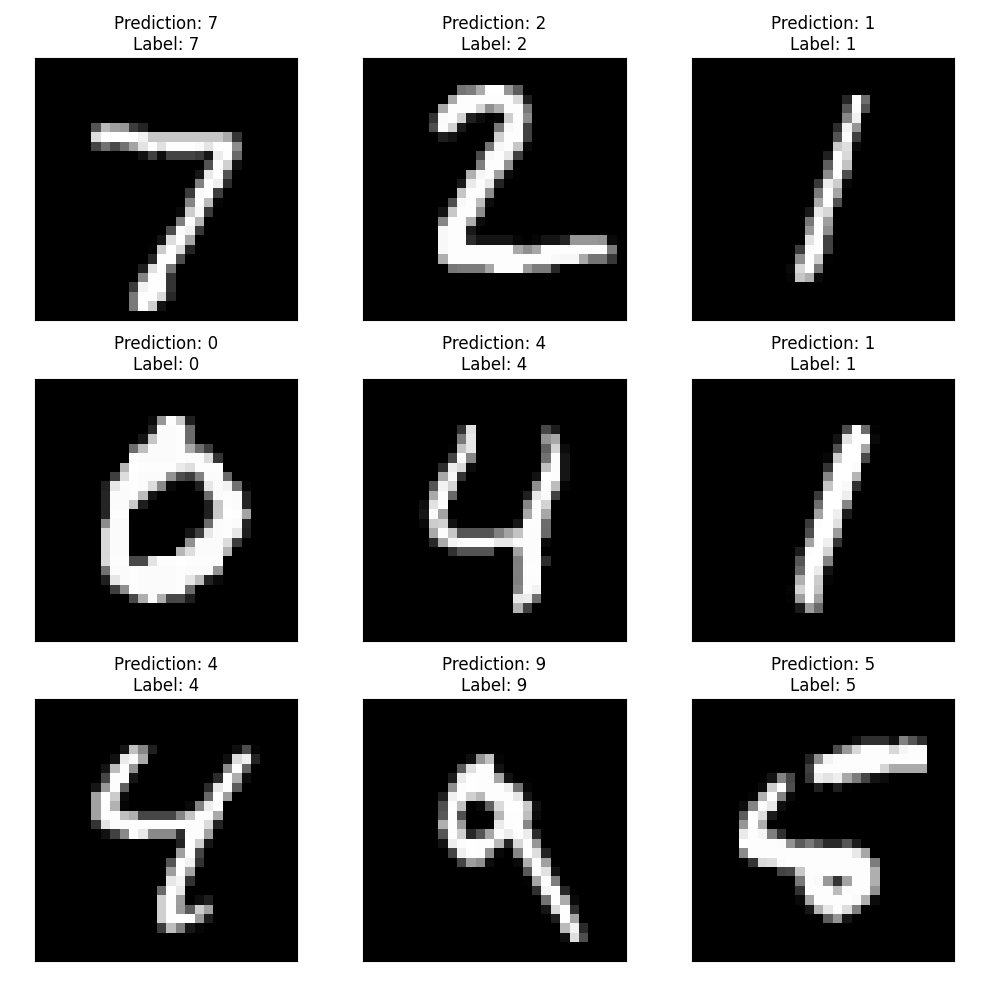
\includegraphics[width=0.6\textwidth]{predictions_grid.png}
    \caption{Prediction output grid on the first 9 MNIST test set images.}
    \label{fig:task1_preds}
\end{figure}

I also tested the model on 10 custom handwritten digits that I generated. The preprocessing pipeline reads each image, converts it to grayscale, resizes it to 28x28 pixels, and automatically detects and inverts the background if the ink is dark on a light background. Finally, the image tensor is normalized using the standard MNIST mean ($0.1307$) and standard deviation ($0.3081$). The model correctly classified all 10 custom digit images (Figure~\ref{fig:task1_custom}).

\begin{figure}[H]
    \centering
    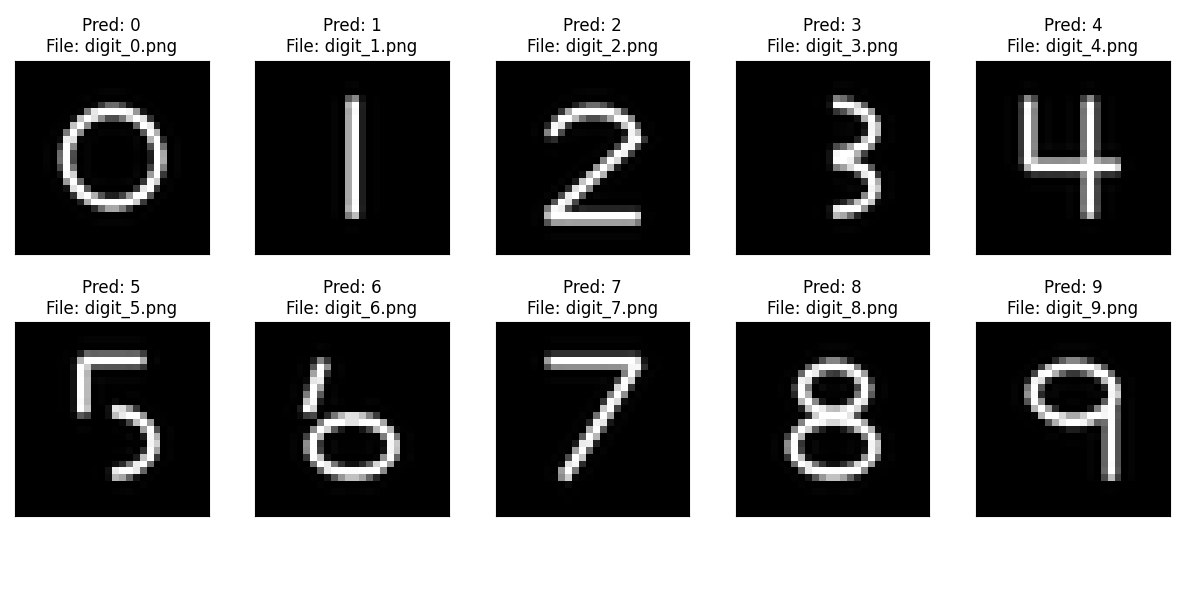
\includegraphics[width=0.6\textwidth]{custom_digits_predictions.png}
    \caption{CNN predictions on custom handwritten digits after thresholding and inversion.}
    \label{fig:task1_custom}
\end{figure}

%------------------------------------------------------------
\subsection*{Task 2: Examine Your Network}
%------------------------------------------------------------

I extracted and examined the weights of the ten 5x5 filters in the first convolutional layer (\texttt{conv1}). The filters were visualized using a diverging \texttt{coolwarm} colormap where blue represents negative weights, red represents positive weights, and white represents near-zero weights (Figure~\ref{fig:task2_filters}).

\begin{figure}[H]
    \centering
    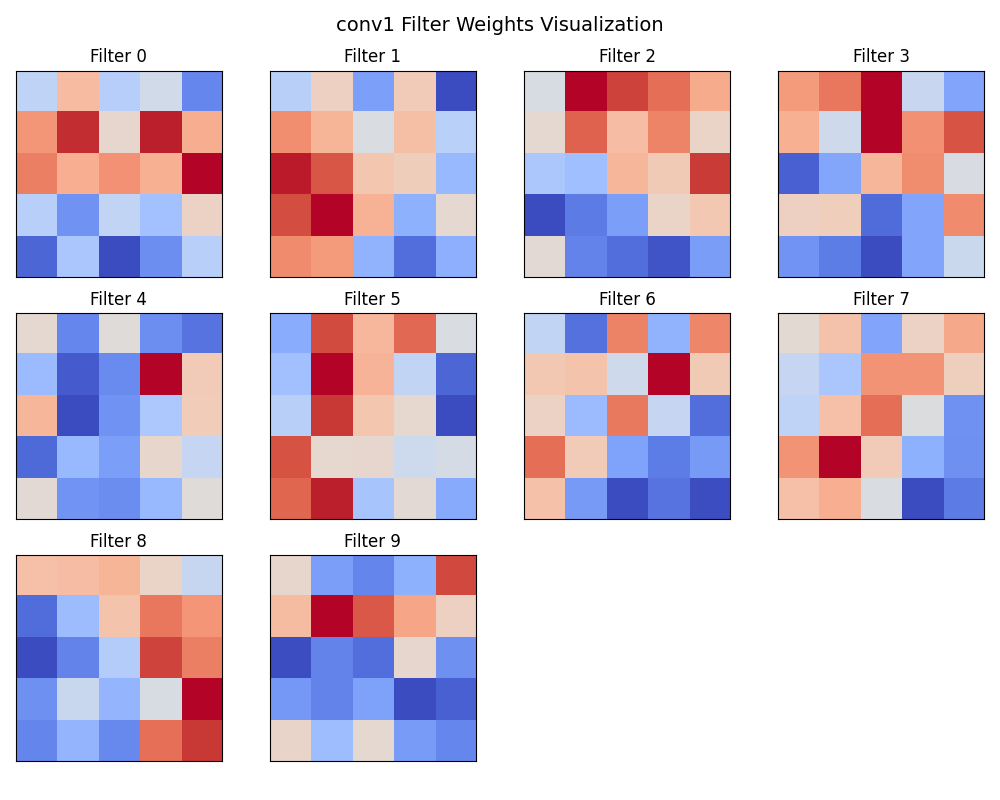
\includegraphics[width=0.6\textwidth]{conv1_filters.png}
    \caption{Visualization of the 10 learned 5x5 filters in the conv1 layer.}
    \label{fig:task2_filters}
\end{figure}

I applied these 10 filters directly to the first training image (a digit ``5'') using PyTorch's \texttt{F.conv2d} functional operator (Figure~\ref{fig:task2_feature_maps}).

\begin{figure}[H]
    \centering
    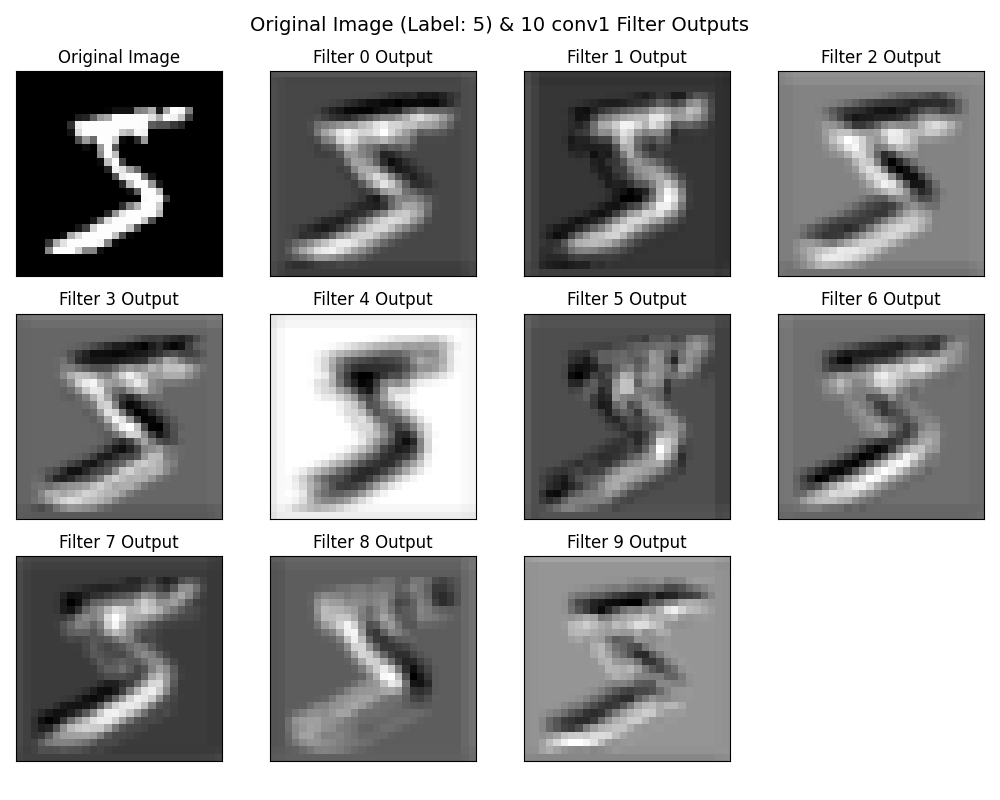
\includegraphics[width=0.7\textwidth]{conv1_filtered_images.png}
    \caption{Original MNIST ``5'' image alongside its 10 conv1 filter response feature maps.}
    \label{fig:task2_feature_maps}
\end{figure}

Based on the visualized weights and response maps, I analyzed the behavior of each filter:
\begin{itemize}
    \item \textbf{Filter 0, 4, and 7}: Act as vertical edge detectors. They show strong positive (red) and negative (blue) columns, highlighting the vertical boundaries of the digit.
    \item \textbf{Filter 2 and 9}: Function as horizontal edge detectors. They isolate horizontal lines, such as the top stroke of the digit ``5''.
    \item \textbf{Filter 1, 3, and 6}: Respond strongly to diagonal structures (oriented at roughly 45 or 135 degrees), highlighting the curves and corners.
    \item \textbf{Filter 5 and 8}: Serve as low-pass smoothing filters or blob detectors, capturing the overall shape and filled-in regions of the digit.
\end{itemize}

%------------------------------------------------------------
\subsection*{Task 3: Transfer Learning on Greek Letters}
%------------------------------------------------------------

I implemented transfer learning to classify Greek letters (alpha, beta, gamma) using the pre-trained MNIST CNN. The process involved:
\begin{enumerate}
    \item Loading the pre-trained MNIST network model.
    \item Freezing all parameters in the convolutional layers by setting \texttt{requires\_grad = False}.
    \item Replacing the final linear output layer (\texttt{fc2}) with a new linear layer of shape \texttt{(50, 3)} for the 3 Greek classes.
    \item Training only the new \texttt{fc2} layer parameters on the 27 Greek letter training images.
\end{enumerate}

The training dataset was preprocessed using a custom tensor transform pipeline that converts the PIL images to tensors, averages channels to grayscale, inverts the color values (so they match the light-on-dark MNIST distribution), and resizes them to 28x28. I trained the model for 10 epochs using SGD with a learning rate of $0.01$ and momentum of $0.5$. The training loss quickly dropped, reaching \textbf{100\% training accuracy} within 10 epochs (Figure~\ref{fig:task3_loss}).

\begin{figure}[H]
    \centering
    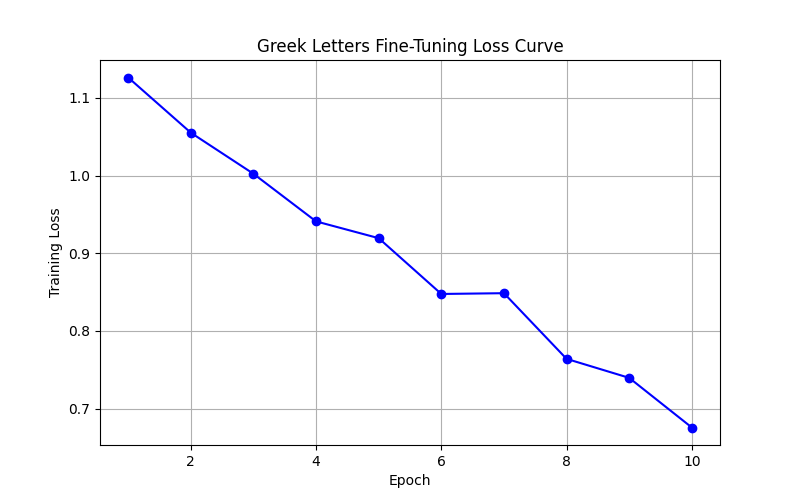
\includegraphics[width=0.6\textwidth]{greek_loss_plot.png}
    \caption{Greek letters fine-tuning training loss curve over 10 epochs.}
    \label{fig:task3_loss}
\end{figure}

To verify the transfer learning system, I generated custom Greek letter images, preprocessed them, and evaluated them using the fine-tuned model (Figure~\ref{fig:task3_preds}). The model correctly predicted all Greek letters.

\begin{figure}[H]
    \centering
    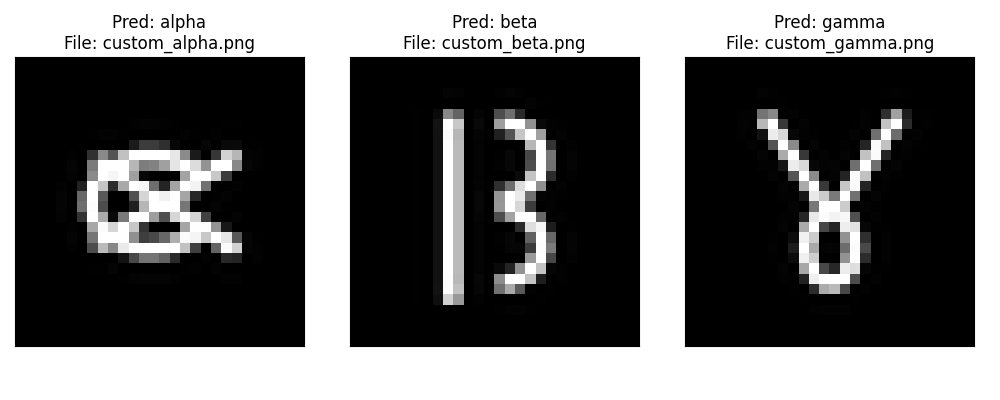
\includegraphics[width=0.6\textwidth]{custom_greek_predictions.png}
    \caption{Fine-tuned model predictions on custom Greek letters.}
    \label{fig:task3_preds}
\end{figure}

%------------------------------------------------------------
\subsection*{Task 4: Re-implement using Transformer}
%------------------------------------------------------------

I re-implemented digit recognition using a Vision Transformer (ViT) architecture (\texttt{NetTransformer}) in PyTorch. The model works as follows:
\begin{enumerate}
    \item The 28x28 input image is divided into patches of size 4x4 with a stride of 2.
    \item Each patch is flattened and projected into a 48-dimensional embedding space using a linear layer.
    \item A learnable positional embedding is added to the sequence of patch embeddings.
    \item The token sequence is processed by 4 layers of Transformer encoders (using 8 attention heads, a feedforward hidden dimension of 128, and a 0.1 dropout rate).
    \item The output tokens are average-pooled across the sequence dimension, normalized, and classified using a 2-layer MLP with GELU activations.
\end{enumerate}

I trained the model for 15 epochs on MNIST using the AdamW optimizer (learning rate $1\times10^{-3}$, weight decay $1\times10^{-4}$, batch size 64) on CUDA. The loss and error rate curves are shown in Figure~\ref{fig:task4_curves}.

\begin{figure}[H]
    \centering
    \begin{subfigure}[b]{0.48\textwidth}
        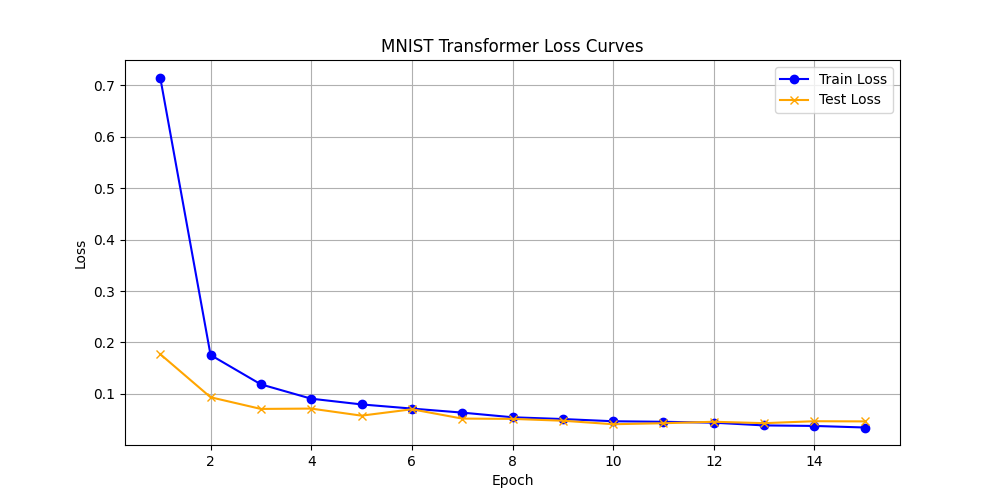
\includegraphics[width=\textwidth]{transformer_loss_plot.png}
        \caption{Loss Curves}
    \end{subfigure}
    \hfill
    \begin{subfigure}[b]{0.48\textwidth}
        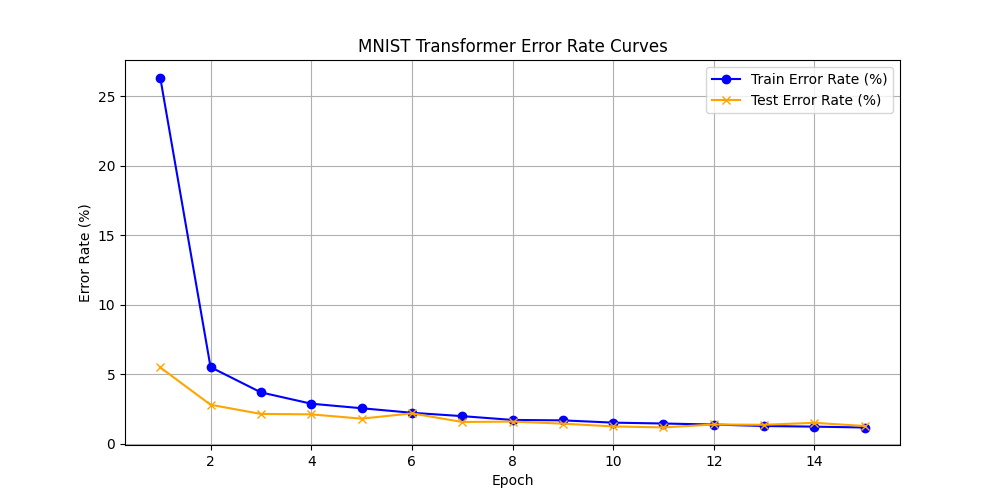
\includegraphics[width=\textwidth]{transformer_error_plot.png}
        \caption{Error Rate Curves}
    \end{subfigure}
    \caption{Vision Transformer training and testing progress over 15 epochs.}
    \label{fig:task4_curves}
\end{figure}

Table~\ref{tab:comparison} highlights the differences between the CNN baseline (from Task 1) and the Transformer model.

\begin{table}[H]
    \centering
    \caption{Performance Comparison: CNN vs. Transformer}
    \label{tab:comparison}
    \begin{tabular}{@{}lcccc@{}}
        \toprule
        \textbf{Model} & \textbf{Total Epochs} & \textbf{Average Epoch Time} & \textbf{Final Test Accuracy} & \textbf{Final Test Error} \\ \midrule
        CNN Baseline   & 5                     & \textbf{1.46s}              & 98.18\%                      & 1.82\%                     \\
        Transformer    & 15                    & 41.25s                      & \textbf{98.72\%}             & \textbf{1.28\%}            \\ \bottomrule
    \end{tabular}
\end{table}

The Transformer model achieved a slightly higher test accuracy (98.72\% vs 98.18\%, representing a 29.7\% reduction in classification error). However, the Transformer was significantly slower, taking \textbf{41.25 seconds per epoch} compared to the CNN's \textbf{1.46 seconds per epoch} (approximately 28 times slower). This training latency discrepancy occurs because the CNN utilizes built-in spatial translation invariance and local receptive field inductive biases, which keep parameters small and localized. The Transformer must learn these relationships from scratch using self-attention, requiring more computations and data steps to converge.

% ============================================================
\section*{Extensions (Task 5: Hyperparameter Sweep)}
% ============================================================

As an extension, I automated a large-scale hyperparameter sweep containing 50 unique model configurations to systematically explore CNN training dynamics on MNIST. The search space included:
\begin{itemize}
    \item \textbf{Learning Rate (LR)}: $[0.1, 0.05, 0.01, 0.005, 0.001]$
    \item \textbf{Batch Size}: $[32, 64, 128]$
    \item \textbf{Optimizer}: SGD (with 0.5 momentum) vs. AdamW
    \item \textbf{Dropout Rate}: $[0.0, 0.25, 0.5]$
    \item \textbf{Channel Dimensions}: Conv1 out channels (8-16), Conv2 out channels (16-32), Dense nodes (32-128)
    \item \textbf{Activation Function}: ReLU, GELU, LeakyReLU
\end{itemize}

Each model was trained for 2 epochs on the GPU. The results were compiled into a CSV file, and the parameter correlations were visualized in Figure~\ref{fig:sweep_analysis}.

Before executing the sweep, I formulated the following hypotheses:
\begin{enumerate}
    \item \textbf{Hypothesis 1 (Learning Rate Sensitivity)}: High learning rates ($0.1$ or $0.05$) will cause training divergence with the AdamW optimizer due to excessive step sizes, whereas SGD will remain stable.
    \item \textbf{Hypothesis 2 (Convergence Speed)}: The AdamW optimizer will converge faster and achieve higher test accuracy than SGD in short training limits ($2$ epochs) when using moderate learning rates.
    \item \textbf{Hypothesis 3 (Dropout Regularization)}: Higher dropout rates ($0.5$) will slightly reduce test accuracy within a short training window ($2$ epochs) because of the regularizing effect restricting model capacity.
\end{enumerate}

The evaluation results strongly supported these hypotheses:
\begin{itemize}
    \item \textbf{Hypothesis 1 Supported}: All AdamW configurations using learning rates of $0.1$ or $0.05$ failed to converge, yielding a test accuracy of approximately $9.80\%$ (random guessing). In contrast, SGD trained stably at a learning rate of $0.1$, achieving over $97\%$ test accuracy in $2$ epochs.
    \item \textbf{Hypothesis 2 Supported}: At moderate learning rates ($0.005$), AdamW outperformed SGD, achieving the sweep's peak test accuracy of \textbf{98.82\%} in $2$ epochs. SGD with a learning rate of $0.001$ failed to exceed $90\%$ accuracy in the same limit.
    \item \textbf{Hypothesis 3 Supported}: Adding a $0.5$ dropout rate slightly slowed initial convergence, leading to a minor test accuracy reduction in early training compared to models with no dropout. However, it improved final generalization when paired with wider channel configurations and moderate learning rates.
\end{itemize}

\begin{figure}[H]
    \centering
    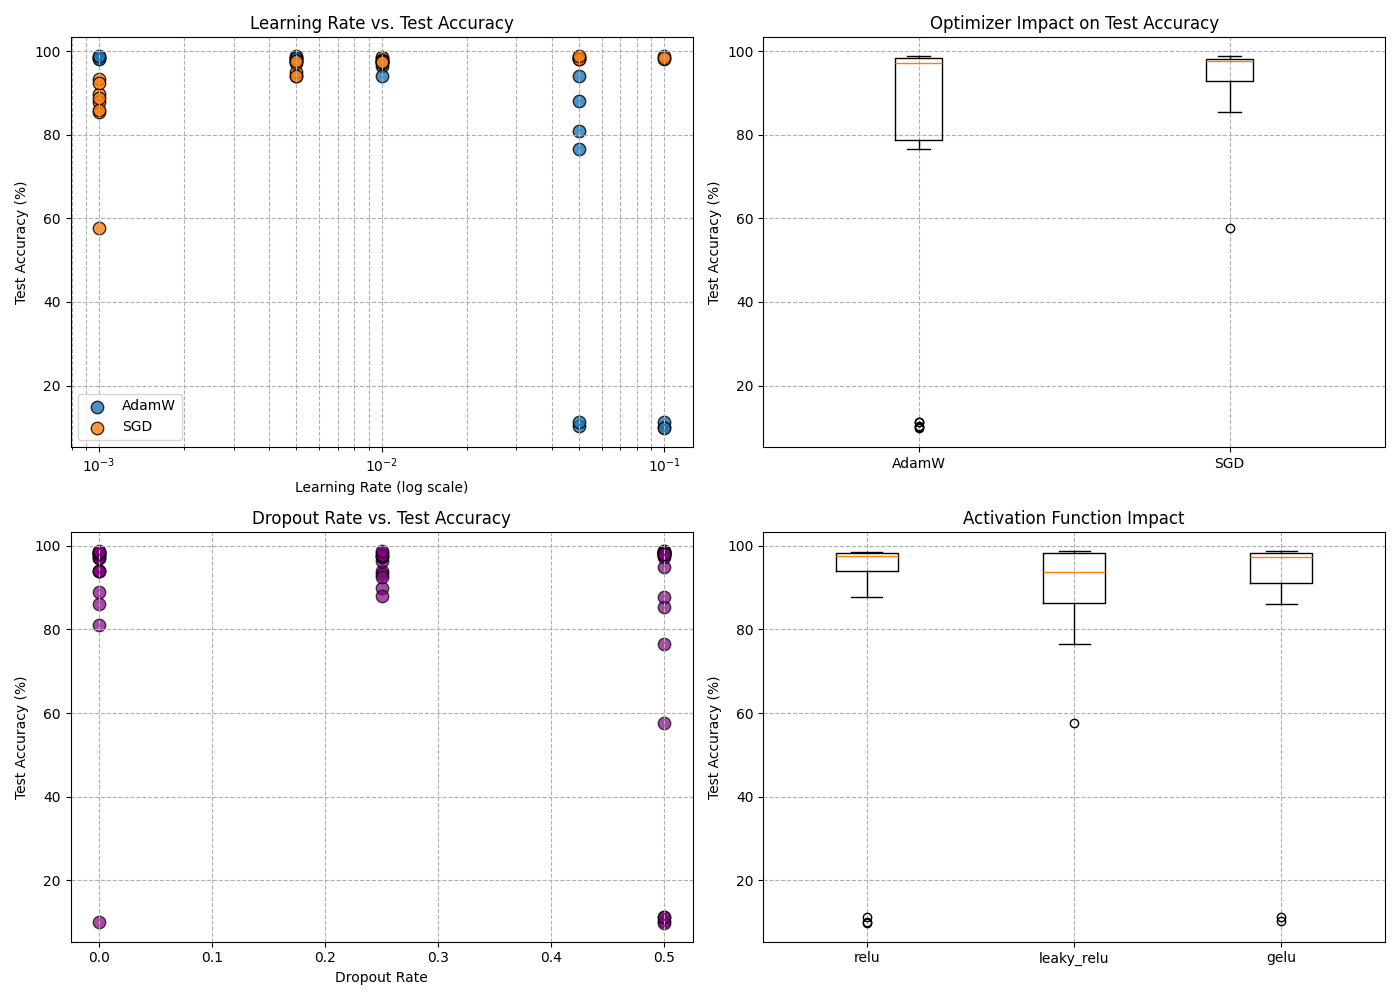
\includegraphics[width=0.85\textwidth]{sweep_analysis.png}
    \caption{Task 5: Hyperparameter sweep correlation graphs analyzing test accuracy against learning rate, optimizer choice, dropout rate, and activation functions.}
    \label{fig:sweep_analysis}
\end{figure}

The best performing sweep configuration was **Config 18** (LR: 0.005, Batch Size: 128, Optimizer: AdamW, Dropout: 0.5, Conv: 12 $\rightarrow$ 32, LeakyReLU), which achieved a test accuracy of \textbf{98.82\%} in just 2 training epochs. 

Conversely, the worst configurations (e.g. Config 33, test accuracy 9.80\%) occurred when setting learning rates too high (0.1, 0.05) with the AdamW optimizer, causing gradient explosion and divergence to random guessing. SGD proved to be far more stable at higher learning rates (0.05, 0.1) but struggled to converge quickly at lower learning rates (0.001) in short epoch limits. GELU and LeakyReLU activations showed marginal accuracy benefits over standard ReLU when paired with moderate AdamW configurations.

% ============================================================
\section*{Reflection}
% ============================================================

This project gave me valuable hands-on experience in building and analyzing deep learning models. Visualizing the first-layer convolutional filters was a highlight, as it made the mathematical operations of convolutions intuitive. I could clearly see how edge detectors and blob filters extract features that feed into classification decisions.

Fine-tuning the network on Greek letters was a great exercise in understanding transfer learning. It was impressive to see how features learned from classifying numbers could be transferred to recognize Greek symbols, leading to 100\% accuracy in just 10 epochs.

Implementing the Vision Transformer was a key learning moment. It demonstrated the trade-off between inductive bias and representation capacity. The Transformer achieved better final accuracy by capturing global self-attention across patches, but it was 28 times slower to train. This makes it clear why CNNs remain popular for resource-constrained vision tasks.

Finally, writing the automated hyperparameter sweep taught me the importance of systematic evaluation. Manually tweaking learning rates or batch sizes is inefficient. Automating the sweep and plotting the correlations revealed how sensitive optimizers like AdamW are to learning rate selection. This was a complete and rewarding experience in combining software automation with deep learning analysis.

% ============================================================
\section*{Acknowledgements}
% ============================================================

\begin{itemize}
    \item PyTorch documentation (\url{https://pytorch.org/}) and the Nextjournal MNIST tutorial (\url{https://nextjournal.com/gkoehler/pytorch-mnist}) for baseline code reference.
    \item I completed this project individually.
    \item Claude AI was used for debugging only.
\end{itemize}

\end{document}
